\documentclass[Afour,times,sagev]{sagej}
\usepackage{url}

\long\def\comment#1{}

\begin{document}
\runninghead{A. Hori and K. Yoshinaga, et al.}
\title{Overhead of Using Spare Nodes}
\author{Atsushi Hori\affilnum{1}, 
  Kazumi Yoshinaga\affilnum{1},
  Thomas Herault\affilnum{2},
  Aur\'elien Bouteiller\affilnum{2},
  George Bosilca\affilnum{2},
  Yutaka Ishikawa\affilnum{1}}

\affiliation{\affilnum{1}RIKEN Advanced Institute for Computational Science\\
\affilnum{2}The University of Tennessee, Innovative Computing Laboratory}

\corrauth{A. Hori, 7-1-26 Minatojima-minami-machi, Chuo-ku, Kobe,
  Hyogo, JAPAN. 650-0047}

\email{ahori@riken.jp}

\begin{abstract}

With the increasing fault rate on high-end supercomputers, the topic
of fault tolerance has been gathering attention. To cope with this
situation, various fault-tolerance techniques are under
investigation; these include user-level, algorithm-based
fault-tolerance techniques and parallel execution environments that
enable jobs to continue following node failure. Even with these
techniques, some programs with static load balancing, such as
stencil computation, may underperform after a failure recovery. Even
when spare nodes are present, they are not always
substituted for failed nodes in an effective way.
This paper considers the questions of how spare nodes should be
allocated, how to substitute them for faulty nodes, and how much the
communication performance is affected by such a substitution.
The third question stems from the modification of the rank mapping by
node substitutions, which can incur additional message collisions.
In a stencil computation, rank mapping is done in a
straightforward way on a Cartesian network without incurring any
message collisions. However, once a substitution has occurred, the
optimal node-rank mapping may be destroyed. Therefore, these questions
must be answered in a way that minimizes the degradation of
communication performance.
In this paper, several spare-node allocation and node-substitution
methods will be proposed, analyzed, and compared in terms of
communication performance following the substitution. Several
substitution methods are proposed and named sliding methods. The
proposed methods are analyzed by using our developed simulation
program and evaluated by using the K computer, BG/Q and TSUBAME
2.5. It will be shown that when a failure occurs, the stencil
communication performance on the K and BG/Q can be slowed around ten
times depending on the number of node failures.  
The barrier performance on the K can be cut in half. On
BG/Q, barrier performance can be slowed by a factor of ten. 
Further, it will also be shown that no communication performance
degradation with failed node substitution can be seen on TSUBAME 2.5
has Fat-Tree network, while the K computer and BG/Q
have Cartesian networks. Thus, the communication performance
degradation depends on network topology.
\end{abstract}

\keywords{fault tolerance, fault mitigation, spare node, communication
  performance}

\maketitle

\section{Introduction}

With the fault rate increasing on high-end supercomputers, the topic
of fault tolerance has been gathering attention\citep{techrep10040},
and jobs are being aborted due to system errors\citep{6903615}. To cope
with this situation, various fault tolerance techniques have been
investigated. Checkpoint and restart is a well-known technique for
parallel jobs, and enabling jobs to continue execution from a
previously defined checkpoint (there are many studies ans systems of
checkpoint and restart, but the most notable one is CLIP\citep{CLIP}).

With the increase in size of parallel applications, the total amount
of I/O needed for checkpoint/restart begun to be problematic. A lot of 
research is currently going on on techniques to reduce the checkpoint
amount in order to alleviate the I/O issue
(Sato\citep{Sato:2012:DMN:2388996.2389022}, for example). On the other
hand, user-level
checkpoints, where each program implements its own checkpoint/restart
strategy, have been attracting attention as a possible
alternative. Since the user knows which data should be saved and which
data can be lost, the amount of checkpoint data can be drastically
reduced, and thus the I/O time can also be greatly reduced, at the
cost of only some additional programing by the user.

Davies {\it et al.} presented a method that allows a user program to
be fault-tolerant without using
checkpointing\citep{Chen:2008:AFT:1477064.1477361}. In this
technique, the parity to recover the lost data can be embedded into an
LU decomposition algorithm, and the user program can recover from
failure without checkpointing. Having the opportunity to address the
failure at the algorithm level opens interesting perspective and new
research topics. With support from the programing paradigm and the
execution environment, users could write application handling faults
in the most optimal way. The Message Passing Interface (MPI) is the
most widely used communication library, and its specifications are
well defined\citep{mpi-v3}. Unfortunately, in the current MPI standard,
a fatal error handler is raised upon process failure, preventing any
user-level fault handling to be implemented at this time.

To define the behavior of MPI when a fault occurs, User-level Failure
Mitigation (ULFM) has been proposed and a prototype is being
developed, capable of handling both process and node
failures\citep{Bland01082013}. ULFM provides the application program
interface (API) so that the modifications to the existing MPI
specifications are minimized. Even with ULFM, user-level fault
handling is not straightforward, and various frameworks have been
proposed to simplify it. Falanx is a fault-tolerant framework for
master-worker programing\citep{falanx}. Local Failure Local Recovery
(LFLR) is another fault-tolerant
framework\citep{Teranishi:2014:TLF:2642769.2642774}, and it covers a
wider range of programing models than are supported by Falanx. Both
Falanx and LFLR are implemented by using ULFM. Global View Resilience
(GVR) is another user-level fault mitigation system; it is based on
partitioned global address space (PGAS)
programing model\citep{gvr-sc14,GVR-vecpar2014}.

We believe that the user-level fault-handling code must be as simple
as possible. It is important to avoid situations in which the code for
handling the first node failure is different from the code for
handling subsequent failures, because it is very hard to produce this
type of situation when testing a program. This type of complexity must
be hidden within the system software.

\begin{figure}[ht]
\centering
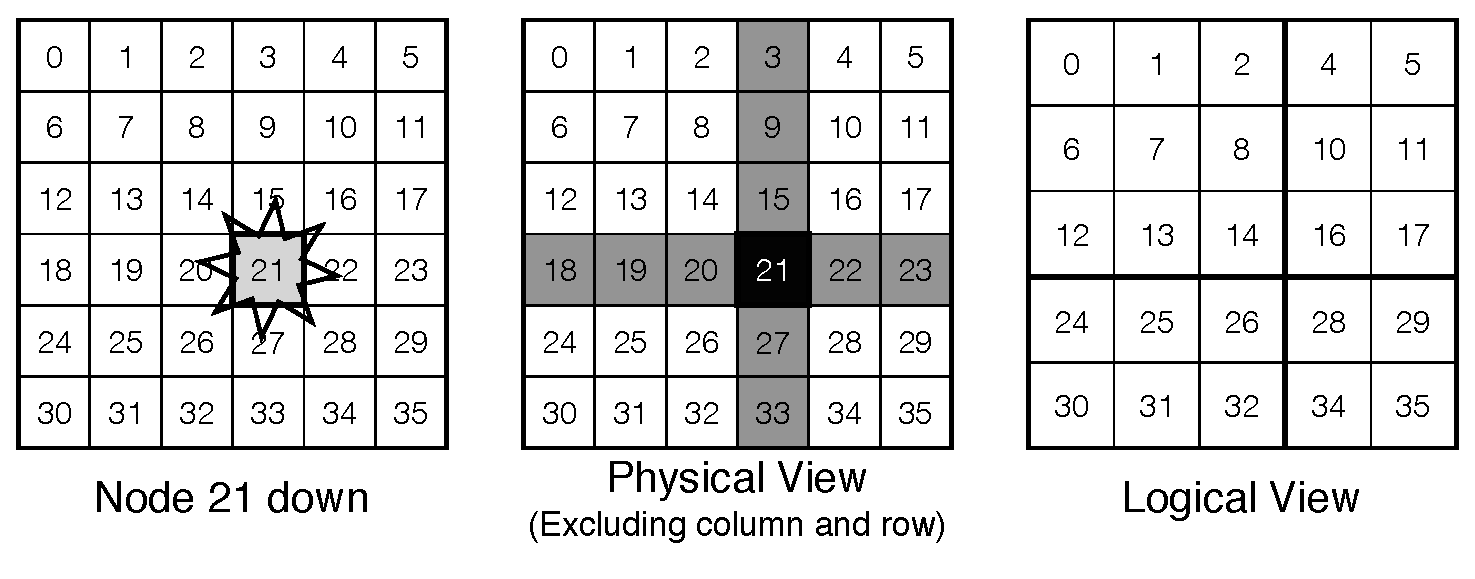
\includegraphics[width=80mm]{Figs/NodeFailure.eps}
  \caption{Example of node failure and recovery}
  \label{fig:node-failure}
\end{figure}

Figure \ref{fig:node-failure} shows an example of a node failure in a
2D network consisting of 36 nodes. Here, it is assumed that a job is
running on this machine, and the job is written with a fail-stop-free
runtime system, such as ULFM. When node 21 goes down (left panel in
Figure \ref{fig:node-failure}), the job running on those 36 nodes can
take one of the following actions:

\begin{itemize}
\item Abort the job and resubmit it (from a previous
  checkpoint, if possible), or
\item Allow the remaining 35 nodes to continue to execute the job.
\end{itemize}

In the first strategy, user-level fault handling is not required.
In the second strategy, the task allocated to the failed node must
be equally shared by the remaining 35 nodes, otherwise, a load
imbalance occurs. If the job can balance a dynamic load, which is a
capability of master-worker models and particle-in-cell simulations,
then the load can be rebalanced by the application itself, without the
need to extensively modify the code. However, if the job is a stencil
application, which, in most cases, does not have dynamic load
balancing capability, then fault handling is more difficult. In most
stencil applications, both the communication pattern and the load
balancing are static. To preserve the communication pattern, one
possibility for handling a node failure is to exclude the row and
column that include the failed node (middle panel in Figure
\ref{fig:node-failure}); this preserves the stencil communication
pattern. However, the task allocated to the failed node must be shared
equally by the remaining nodes (right panel in Figure
\ref{fig:node-failure}). This load-leveling requires additional code
for handling the fault, and this must be avoided if possible.

If a system software reserves a set of spare nodes in advance, and the
failed node is replaced by a spare node, then the user-level handling of
node failure is simplified, because the number of nodes involved in
the computation remain the same. LFLR assumes the use of spare nodes,
and although the detailed recovery process is hidden from users, GVR
may utilize spare nodes. However, to the best of our knowledge, there
has been no discussion of the best way to reserve spare nodes or of
how to use them to replace failed nodes. As an evaluation index, we
chose communication performance, because the use of spare nodes may
introduce extra message collisions.

This paper presents the results of our investigations into these
issues. As a first step to address these issues, we propose several
methods for using spare nodes to replace faulty ones in addition to
the spare node allocations. The proposed methods are discussed and
compared from the viewpoint of communication performance
degradation. The contributions of this paper are;  

\begin{itemize}
\item spare node allocation methods are proposed,
\item failure node substitution methods are proposed,
\item focusing on stencil communication and some collective
  performance, the behaviour and characteristics of proposed spare
  node allocation and substitution methods are revealed by simulations, and
\item evaluations on the two supercomputers having a Cartesian network
  topology and one supercomputer having a FatTree network topology take
  place to see how a network topology affects the communication
  performance degradation
\end{itemize}

\section{Using Spare Nodes}

For the remainder of this paper, we will assume that the networks
being considered have a multidimensional Cartesian (mesh and/or torus)
topology, otherwise noticed. We make this assumption because four of
the top five machines have networks with this topology (as listed on
the TOP500 Super Computer Site\citep{top500}, November
2015); see Table \ref{tbl:top5-network}. 

\begin{table}[htb]
\centering
\caption{Network topologies in the Top500 list\citep{top500}}
\label{tbl:top5-network}
{\small
\begin{tabular}{c|l|r|l}
\hline
Top500 & &  & \\
rank & Name & \# Cores & Topology \\
\hline
\hline
1 & Tianhe-2 & 3,120K & FatTree \\
2 & Titan (Cray XK7) & 561K & 3D Torus \\
3 & Sequoia (BG/Q) & 1,573K & 5D Torus/Mesh \\
4 & The K computer & 705K & 6D Torus/Mesh \\
5 & Mira (BG/Q) & 786K & 5D Torus/Mesh \\
\hline
11 & JUQUEEN (BG/Q) & 459K & 5D Torus/Mesh \\
\hline
25 & TSUBAME 2.5 & 76k (+GPU) & FatTree \\
\hline
\end{tabular}
}
\end{table}

From the programmers point of view, it is not complicated to have
spare nodes held ready, or to have them substituted in for faulty
nodes. With MPI, the modification is as follows: 1) a new MPI
communicator is created at the location from which the faulty node is
extracted (in ULFM, the command {\tt MPI\_Comm\_shrink} will do this),
and a selected spare node replaces the faulty node; 2) the spare node
is set up to take over the functions of the failed node. The remaining
parts of the program can remain as they were. This means that the
logical topology provided by the new MPI communicator can remain the
same as it was before the failure; however, the actual physical
topology is altered. New message collisions that would not
have happened under the failure free physical topology will happen
under the recovered topology (Figure \ref{fig:collisions}).

Therefore, replacing faulty nodes with spare nodes must be done
carefully in order to minimize the communication performance
degradation. There are many other aspects that should be considered,
such as system utilization, job turn-around time, ease of user
programing, and the framework that needs to be
developed. Unfortunately, almost no research has been done on this
topic, so in this paper, we will focus primarily on the communication
performance.

Throughout this paper, we will be concerned only with the node
failure. Network failures can also occur, but we will assume that this
recovery is the responsibility of the network
itself\citep{Domke:2014:FND:2683593.2683659} (see also Section
\ref{sec:related-work}). The Tofu network, which is used by the K
computer, uses redundant links to detour around failed
nodes\citep{sumimoto-k}. We will assume that a job can survive even
with the failure of one or more nodes when it is operating in a
parallel computing environment that provides a user-level fault
mitigation mechanism, such as ULFM, and any processes running on the
failed node can be recovered from a checkpoint or by using parity with
viable processes. Finally, we will assume that the processes running
on a node can be migrated to any other node.

In the next subsection, we will discuss the allocation of spare nodes, and
the possibility of this degrading the communication performance will be
shown. Then, three methods for substituting a spare node for a faulty
node will be proposed and compared.

\subsection{Spare Node Allocation}\label{sec:spare-alloc}

In this section for simplicity, we will consider only 2D networks with
static XY routing routing\citep{Zhang:2009:CRX:1603897.1605067}.
Figure \ref{fig:sparenode-allocation} shows three different ways of
allocating spare nodes. Each small square represents a node. In the
left panel, the right-hand column is reserved for spare nodes; this
pattern is denoted as {\it 2D(1,1)}. In the middle panel, two sides
(the right-hand column and the bottom row) are reserved for spare
nodes, denoted {\it 2D(2,1)}. In the right-hand panel, two two-node
thick sides (the two right-hand columns and two bottom rows) are
reserved, denoted {\it 2D(2,2)}. In this notation, ``2D'' means that
the allocation applies to the 2D plane, the first number in the
brackets is the number of sides in which spare nodes are reserved, and
the second number is the thickness, number of columns or rows, of a
side of spare nodes reserved.

\begin{figure}[ht]
\centering
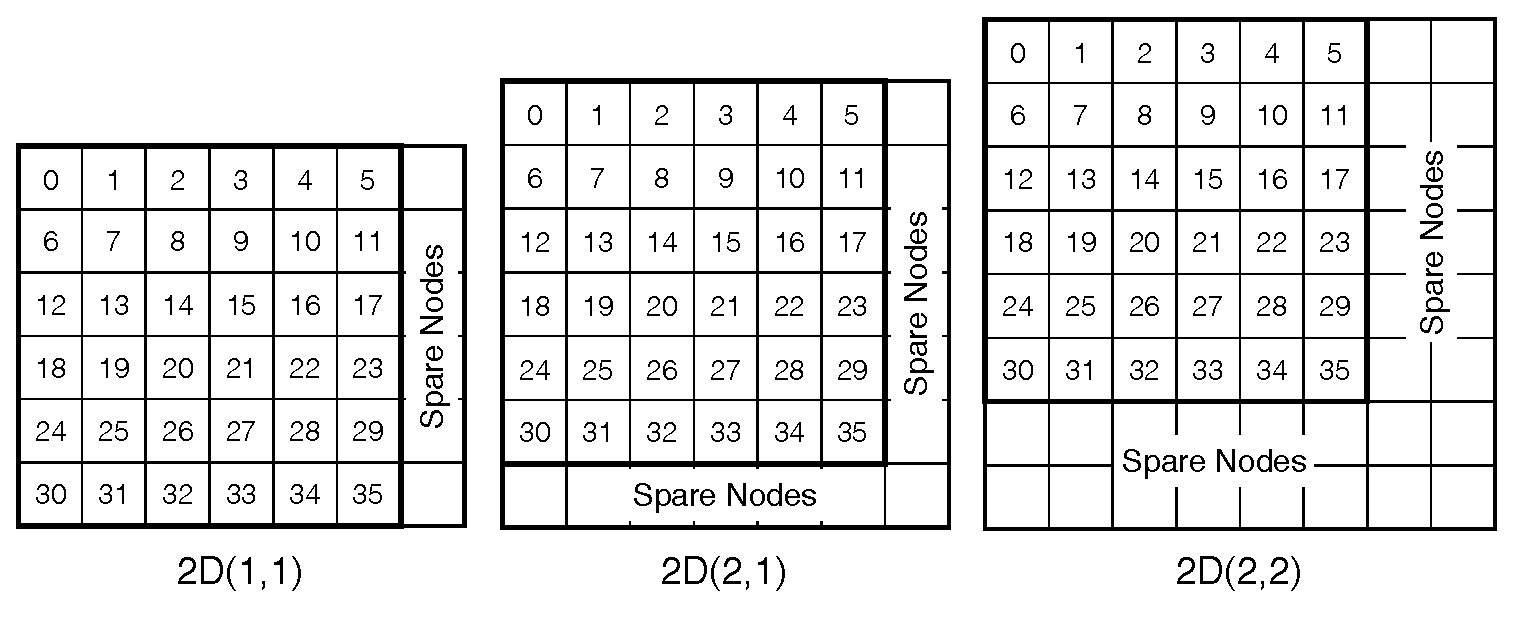
\includegraphics[width=80mm]{Figs/SpareNodeAllocation.eps}
  \caption{Patterns for allocation of spare nodes }
  \label{fig:sparenode-allocation}
\end{figure}

Spare nodes are allocated at the side(s) of a 2D grid, as shown in
Figure \ref{fig:sparenode-allocation}; thus, a stencil application
with non-periodic boundaries will not have any overhead. This will not
be the case for stencil applications that have periodic boundaries or
for networks that have torus topology. However, the hop count is only
increased by one, so the increase in run time will be very small
(100 ns per hop on the K computer).

The percentage of the nodes that are reserved as spare nodes in the
2D(2,2) case is as follows.

\[
R_{2D(2,2)} = 1 - ( N^{1/2} - 2 )^2 / N
\]

Where $N$ is the number nodes. In the more general $qD(r,s)$ case, the
percentage of spare nodes can be expressed as follows.

\[
R_{qD(r,s)} = 1 - \frac{ ( N^{1/q} - s )^r \times ( N^{1/q} )^{q-r} }{ N }
\]

Here, $r \leq q$ and $s < N^q$. Note that this expression is not
precise, because the number of nodes is an integer, and the flooring
effect is ignored. However, this information can be useful for
determining how the spare node percentage relates to the total number
of nodes used for a job.

Figure \ref{fig:sparenode-percentage} shows the percentages of spare
nodes for various numbers of nodes and patterns of allocation. As
shown in this figure, the more dimensions the network has, the higher
the percentage of spare nodes. The percentage is almost proportional
to the number of sides allocated to the spare nodes. Most notably, the
larger the job size, the lower the percentage. We will discuss this
point in Section \ref{label:multi-job}.

\begin{figure}[ht]
\centering
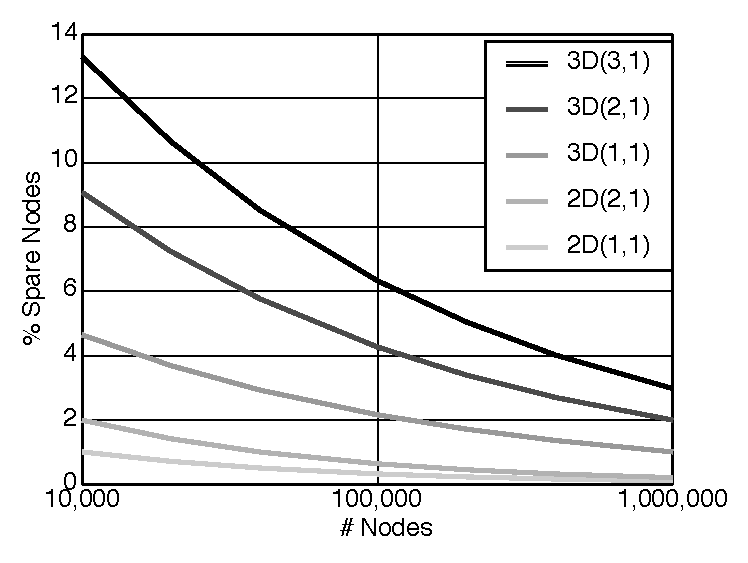
\includegraphics[width=55mm]{Figs/R-SpareNodes.eps}
  \caption{Percentage of spare nodes}
  \label{fig:sparenode-percentage}
\end{figure}

It is possible to allocate spare nodes on four sides of a 2D grid, but
on a torus network, this is almost equal to the 2D(2,2) case. In our
investigation, we could not find any significant difference between
2D(4,1) and 2D(2,2), and so in this discussion, we will not further
consider cases in which $r > q$. The thickness, $s$, does not affect
the nature of the spare node substitution method described in Section
\ref{sec:substitution}, so we will investigate only cases of
single-node thickness.

Having spare nodes can decrease the system utilization ratio. However,
this does not always happen. On the K computer, the size of each
dimension of a job must be in a {\it Tofu unit}, which has twelve
nodes. When a user submits an 11x11x11 3D job, for example, it may be
scheduled to have 12x12x12 nodes. This results in 3D(2,1) spare
nodes. The same situation can be seen with the other machines that
have a Cartesian topology network and are listed in Table
\ref{tbl:top5-network}. On Blue Gene/Q (BG/Q) machines, the number of
nodes for a job must be a power of 2\citep{BGQ-admin}. On a Cray XK/7,
jobs are allocated to $4 \time 2 \time 8$
blocks\citep{Pena:2013:ATM:2488551.2488564}. Thus, the gap between the
number of nodes required by a job and the number of nodes actually
allocated can be allocated as spare nodes, without requiring
additional nodes.

\subsection{Substitution of a Spare Node for a Faulty Node}
\label{sec:substitution}

Communication performance degradation can be observed because when a
spare node that replaces a faulty node can be located far from the
original node. Figure \ref{fig:collisions} shows the 5P-stencil
communication pattern (left). In 5P-stencil communication on a
Cartesian topology, no messages collide, because nodes communicate
only with their neighbors. Here, static XY routing is assumed. In the
right-hand panel of Figure \ref{fig:collisions}, when a faulty node
(denoted as ``F'') is replaced by a spare node (denoted as ``S''), the
regularity of the stencil communication pattern is lost. As shown in
this figure, there are five message routes crossing through the
circled link, this means that up to five messages can collide.

\begin{figure}[ht]
\centering
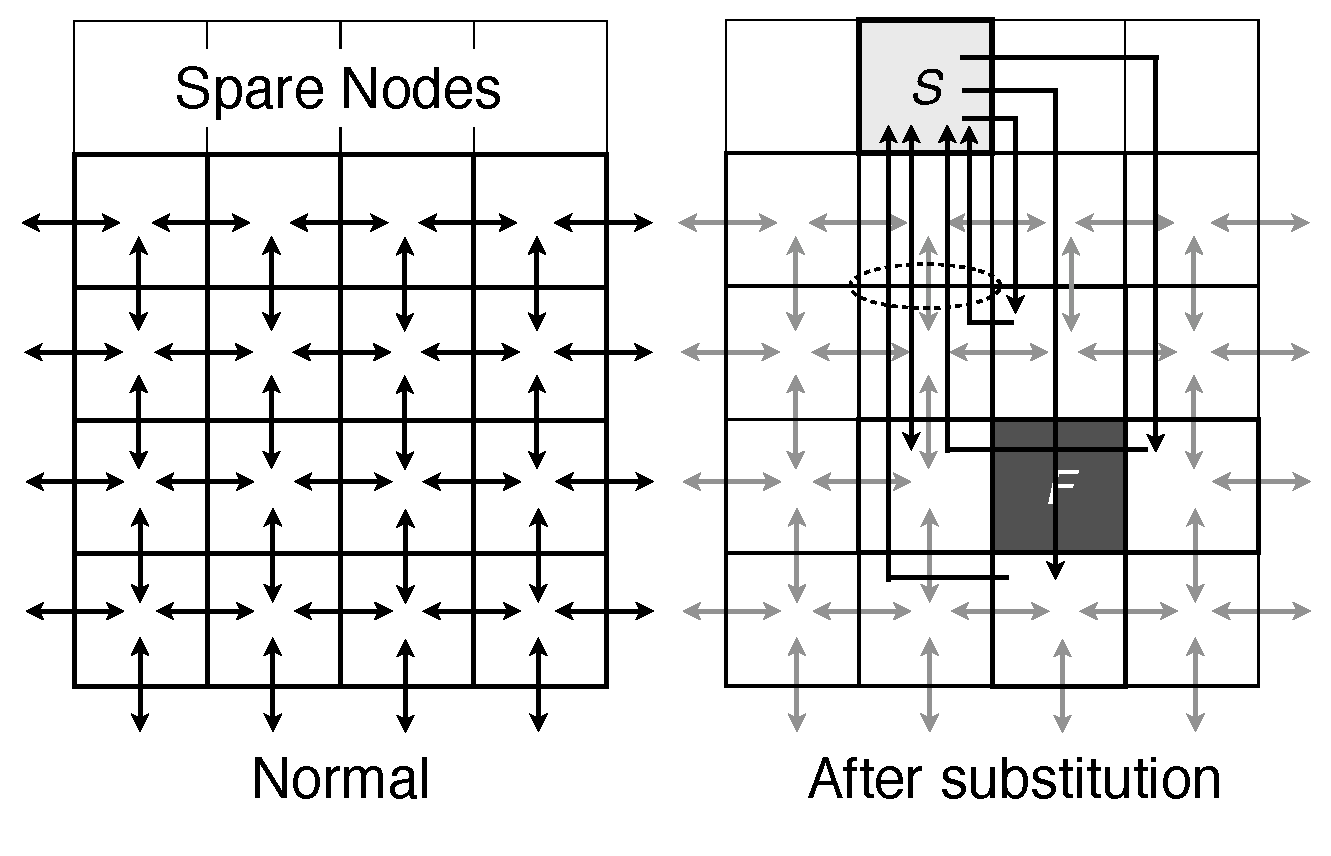
\includegraphics[width=60mm]{Figs/Collision.eps}
  \caption{Message collisions}
  \label{fig:collisions}
\end{figure}

We propose three methods for substituting nodes, and these are shown
in Figure \ref{fig:node-substitution}. We call these methods the {\it
  0D}, {\it 1D}, and {\it 2D} sliding methods. With higher-dimension
networks, those proposed methods can be augmented in a natural way,
but for simplicity, we will explain them on a 2D network. We will use
a 5P-stencil communication pattern, in which messages from each node
are sent up, down, left, and right. In the 9P-stencil communication
pattern, there are an extra four directions, since messages can be
sent along the diagonals. However, in most cases, the length of those
diagonal messages is much shorter than those in a 5P-stencil pattern,
and so the effect on the communication performance is expected to be
small.

\subsubsection{0D sliding}\label{sec:0d-sliding}

The 0D sliding method is the simplest. The faulty node is simply
replaced by a spare node (as was shown in Figure
\ref{fig:node-substitution}). There is a big drawback to this method,
however, when a node failure happens far from a spare node: the hop
distance from the failed node to the spare node can be very
large. This increases the possibility of message collisions and
results in a higher communication latency due to the large number of
hops. To minimize this, the failed node should be replaced with the
spare node to which the Manhattan distance is the shortest.

\begin{figure}[ht]
\centering
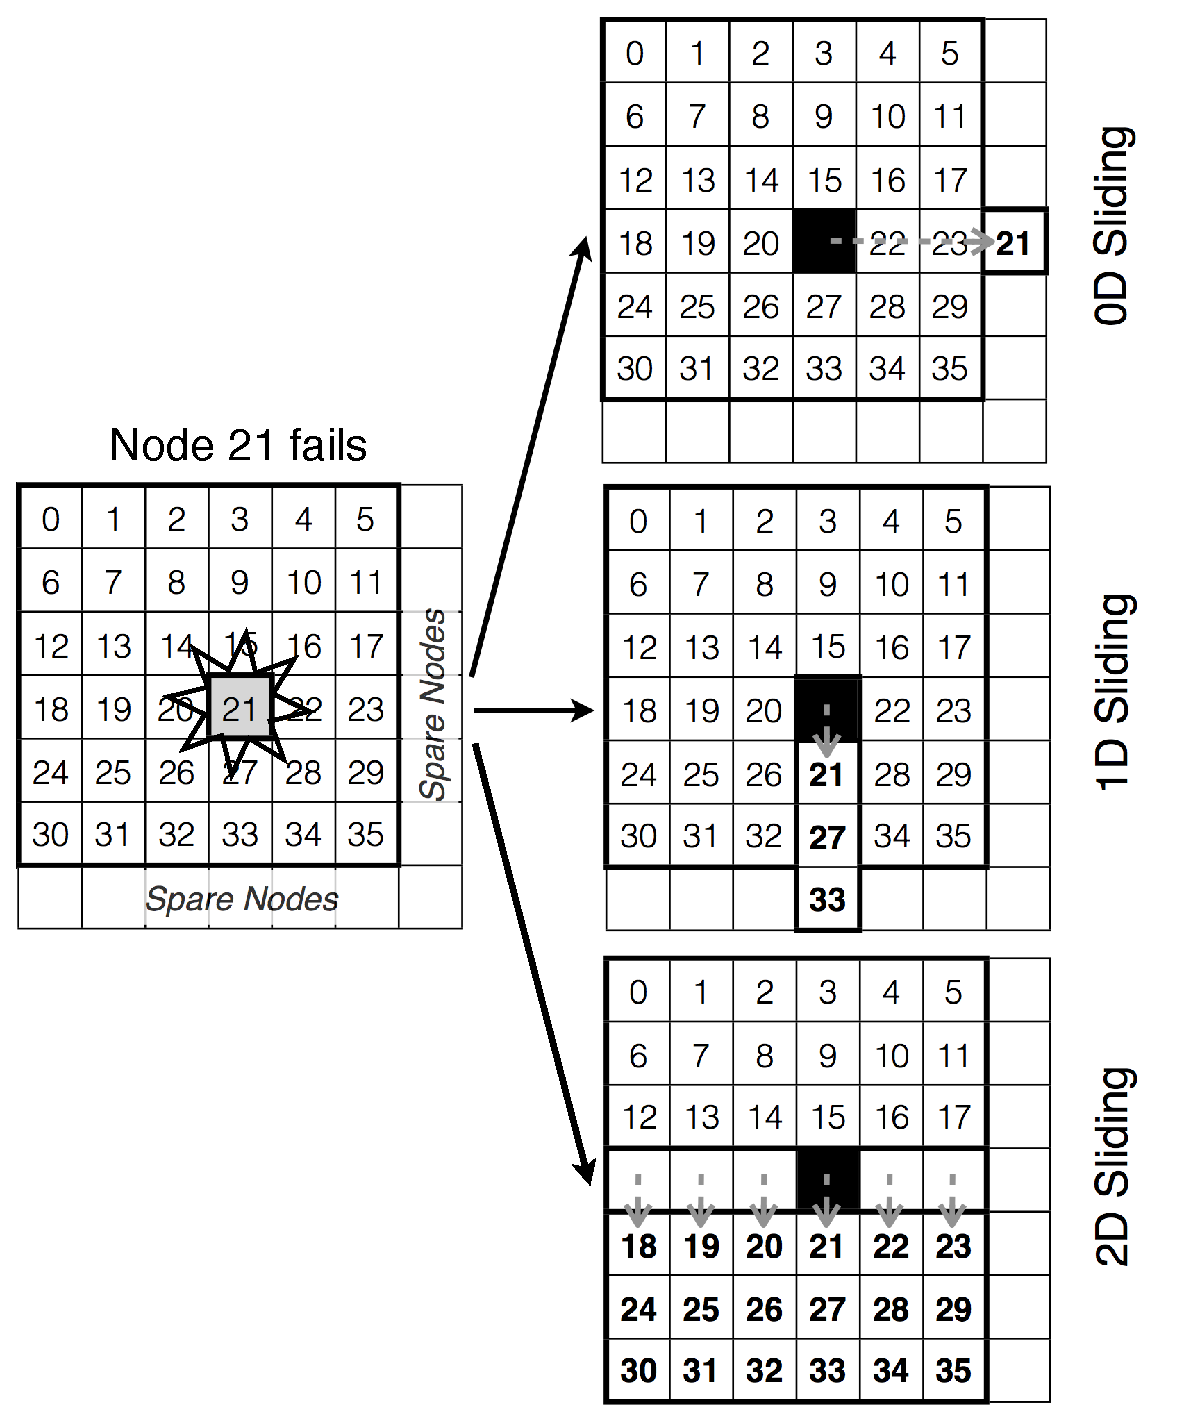
\includegraphics[width=75mm]{Figs/SpareNode.eps}
  \caption{Substitution methods for faulty nodes}
  \label{fig:node-substitution}
\end{figure}

Figure \ref{fig:0d-worst-cases} shows examples of the results of
replacing multiple faulty nodes when using the 0D sliding method with
the 2D(1,1) allocation. On the left-hand panel, nodes 1 through 5 have
failed and have been replaced by spare nodes 1' through 5',
respectively. The spare nodes were chosen so as to minimize the number
of hop counts between each faulty node and its corresponding spare
node. With non-periodic 5P-stencil communication in the XY routing
algorithm, the messages from all of the spare nodes to the nodes (A
through F) adjacent to the failed nodes are routed through node 1'
(because of the X direction routing of the XY routing
algorithm). Thus, there are eleven messages in the network links
between 1' and A  (these are shown in the white boxes): these ten plus
the normal stencil communication message between the nodes. This is
the worst-case scenario for the 0D sliding method, and the number of
faulty nodes is less than or equal to six.

\begin{figure}[ht]
\centering
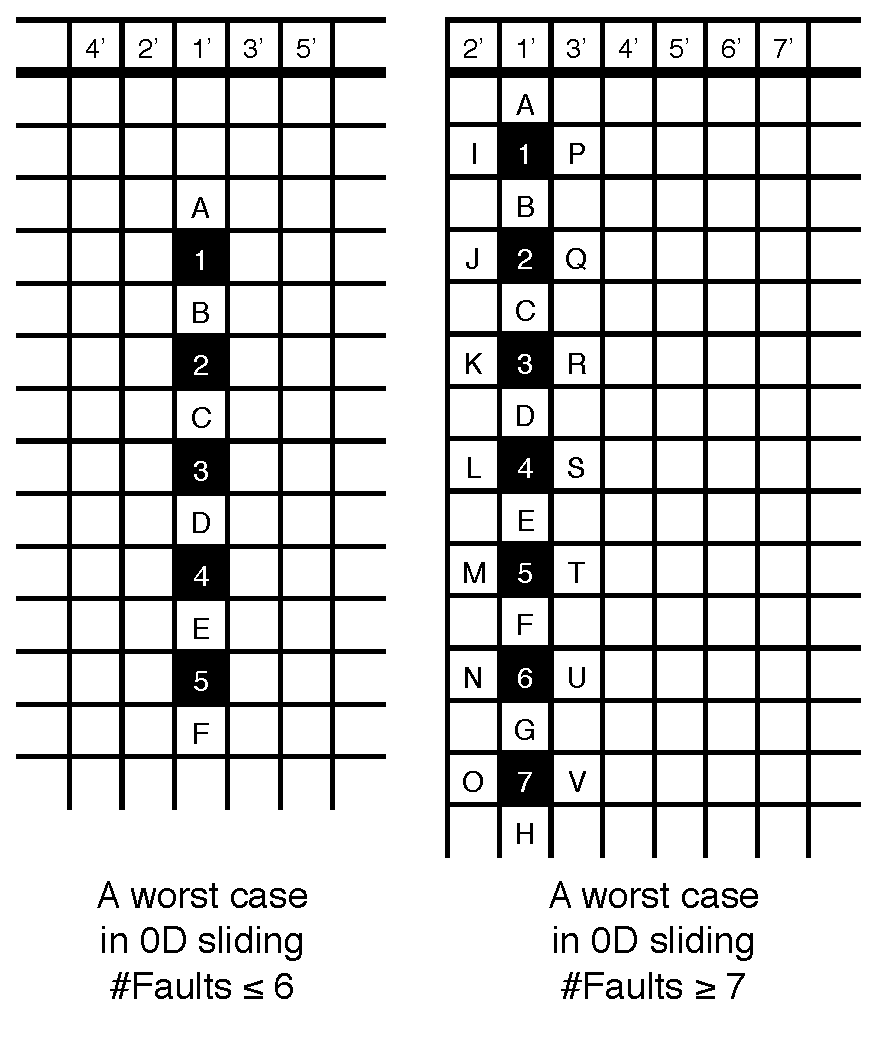
\includegraphics[width=60mm]{Figs/0D-WorstCases.eps}
  \caption{Worst-case scenarios for 0D sliding}
  \label{fig:0d-worst-cases}
\end{figure}

The right-hand panel of Figure \ref{fig:0d-worst-cases} shows a case
for which the network topology is a 2D mesh, spare nodes are reserved
in the 2D(1,1) pattern, and the faults happen within a row or column
that is close to the side of the network. Failed node 1 is replaced by
spare node 1', and so on. In this case, the failures happen close to
the side of the network, and it is not possible to replace the spare
nodes as in the left-hand panel of Figure \ref{fig:0d-worst-cases}. In
non-periodic 5P-stencil communication, all messages from spare nodes
4', 5', 6', and 7' to the neighbor nodes A to V go through the link
between 3' and 4'. There are sixteen messages, since each node sends
four messages, one to each of its neighbor nodes. This situation can
happen when the number of faults is greater than or equal to
seven. Below, we state the relation between the maximum number of
possible message collisions ($C_{max}$) and the number of node
failures ($F_n$). Note that when $C_{max}$ is equal to one, then there
is only one message on each network link, and there are no collisions.

\begin{equation}
C_{max} = \left \{ \begin{array}{ll}
2 \times F_n + 1 & F_n \leq 6~or~torus~topology \\
4 \times ( F_n - 3 ) & F_n \geq 7~and~mesh~topology
\end{array}\nonumber
\right.
\end{equation}

This worst-case scenario can be relaxed by having spare nodes
allocated in the 2D(2,1) pattern. If the failures happen in the same
row or column, then the spare nodes must be chosen from alternating
sides. See Section \ref{sec:comparison}.

\comment{Again, the drawback of the 0D sliding method is the
  possibility of a long distance between the faulty node and the spare
  node. As shown in Figure \ref{fig:0d-K} shown in the next
  subsection, the communication latency was observed to be three times
  larger, and this was almost independent of the number of nodes. This
  phenomenon can differ when the message pattern is not the same as
  that of the 5P-stencil, and When the distance to the replacement is
  considered, the communication performance may be severely degraded
  due to heavy message congestion.}

\subsubsection{1D sliding}

As described in the previous subsection, in the 0D sliding method,
even if the closest spare node is chosen, the distance from the failed
node is unlikely to be small. The 1D sliding method can avoid this
situation, and it is shown in Figure \ref{fig:1d-sliding}. When node
21 fails, instead of replacing it with a spare node, the nodes of the
column (or row) that include the failed node shift toward a
spare node, as shown in the upper left-hand panel of the figure. In
this way, the hop count in the 5D-stencil communication pattern is
increased by only one. This is much smaller than occurs with the 0D
sliding method.

\begin{figure}[ht]
\centering
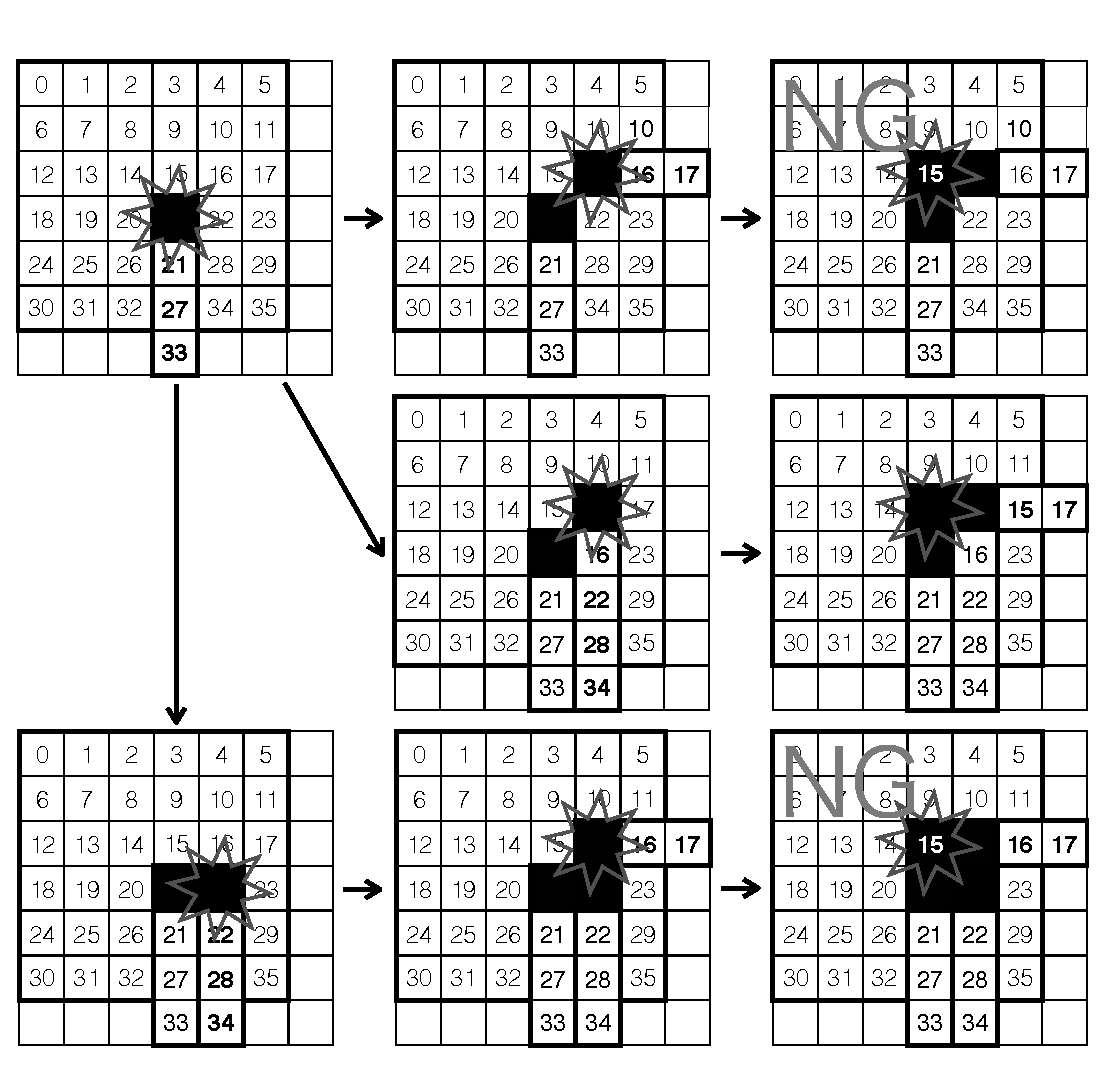
\includegraphics[width=70mm]{Figs/1D-Sliding.eps}
  \caption{Example of 1D sliding}
  \label{fig:1d-sliding}
\end{figure}

In terms of hop counts, the 1D sliding method is superior to the
0D sliding method; however, the recoverable number of faulty nodes is
limited in some cases. Let us consider a case in which a second node
(16) fails (again using the 2D(2,1) pattern); this is shown in Figure
\ref{fig:1d-sliding}. This time, and the sliding direction is along
the column. If a third node (15) fails, then there is no space left
for the 1D sliding (top row of Figure \ref{fig:1d-sliding}). This
situation can be avoided by sliding along the column direction after
the second failure (middle row of Figure \ref{fig:1d-sliding}).

The number of nodes below which a third failure cannot be handled by
the 1D sliding method is the product of the number of slidings in each
direction. Thus, it is not a good idea to evenly distribute the
sliding directions; instead, they should be as uneven as possible.
\comment{(see the sample program codelet in Figure \ref{fig:1d-prog})}
Even when this is done, however, the 1D sliding method may be limited
to three failures (bottom row in Figure \ref{fig:1d-sliding}).

\comment{
\begin{figure}[ht]
\small\tt
\begin{verbatim}
bool try_1D_slide( Node fnode ) {
    if ( try_1D_slide_X( fnode) ) {
        return true;
    }
    if ( try_1D_slide_Y( fnode ) ) {
        return true;
    }
    /* more dimension(s) may follow */
    return try_0D_slide( fnode );
}
\end{verbatim}
\caption{C program for 1D sliding}
\label{fig:1d-prog}
\end{figure}
}

The relation between the maximum number of message collisions and the
number of failed nodes with the 2D(2,1) spare node allocation pattern
can be expressed as shown below. Note that there may be cases in which
this method cannot handle more than three node failures.

\[
C_{max} = 2 + F_n
\]

\subsubsection{2D sliding, 3D sliding, ..., $q$D sliding}

In the 2D sliding method, the rows and columns of the node space are
shifted by one unit to empty the row or column of the failed node
(bottom panel of Figure \ref{fig:node-substitution}). This 2D sliding
method can handle only one node failure with the 2D(1,1) pattern or
two node failures with the 2D(2,1) pattern. 

If the network has a
higher-dimensional Cartesian topology than 2D, then the 3D or
higher-order sliding can take place in the same way. The highest
degree of a sliding method is equal to the number of dimensions of a
Cartesian network and this sliding method can handle up to the number
of dimensions. 

With XY routing, the messages pass orthogonally through the vacant
rows or columns. All message routes are the same as they were before
the failure. Thus, unlike the 0D and 1D sliding methods, although the
hop counts are increased by one, message congestion can be
avoided. Further, this behavior is independent of the communication
pattern of the application.

\subsection{Comparison of Proposed Methods}\label{sec:comparison}

Figure \ref{fig:comparison} shows the number of possible message
collisions versus the number of failed nodes for the 0D sliding method
with the 2D(1,1) and 2D(2,1) spare node allocation patterns, 1D
sliding with the 2D(2,1) pattern, and 2D sliding with the 2d(2,1)
pattern. These numbers are obtained by our developed simulation
program with which every possible combinations of node failures is
simulated so that the number of message collisions in a 5P-stencil
communication are counted at every link and the highest number of
message collisions is reported. In this simulation, it is assumed that
four messages of 5P-stencil communication are sent simultaneously. 

\begin{figure}[ht]
\centering
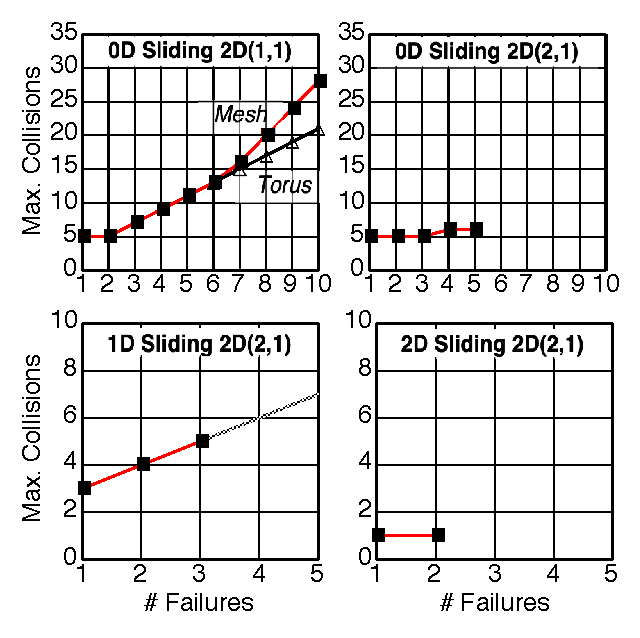
\includegraphics[width=70mm]{Figs/SmallN-Failures.eps}
  \caption{Comparison of 0D, 1D, and 2D sliding (5P-stencil, worst
    cases with exhaustive search)}
  \label{fig:comparison}
\end{figure}

As already described in Section \ref{sec:0d-sliding}, the number of
possible message collisions with 0D sliding with the 2D(1,1)
allocation pattern for a given number of failed nodes depends on the
network topology (mesh or torus) when the number of faults is greater
than six (upper left-hand panel in the figure). With 2D(2,1) case, up
to 5 failures are simulated. It is possible to handle more number of
failures with the 0D sliding method, however, the exponential growth
of failure combinations was the obstacle for us to simulate more.

The 1D sliding method with the 2D(2,1) spare node allocation pattern
can handle up to three failures perfectly. More number of failures can
be handled when the failures happen at some specific locations. This
is shown as a dashed line in Figure \ref{fig:comparison}.

The 1D sliding method can handle no more than the number of
spare nodes minus one, since the spare node at the corner of the
2D(2,1) allocation cannot be used. The 2D sliding with 2D(2,1) can
handle only two failures as described before.

The sliding method has a good characteristic where node migration can
take place in a pipeline fashion. Therefor the time to migrate nodes
can be independent ($O(1)$, assuming the amount of data to be migrated
are the same over nodes) from the number of migrating nodes.

\subsubsection*{Hybrid method}

The substitution methods described so far are independent and can be
applied in a combined way. Figure \ref{fig:hybrid-sliding} shows an
example of a hybrid method. The first and second failures are handled
by using the 2D sliding method (left-hand and middle panels), and the
third failure is handled by using the 1D sliding method (right-hand
panel). In this way, message collisions can be avoided even up to two
failures, and the job can survive even with a greater number of
failures.

\begin{figure}[ht]
\centering
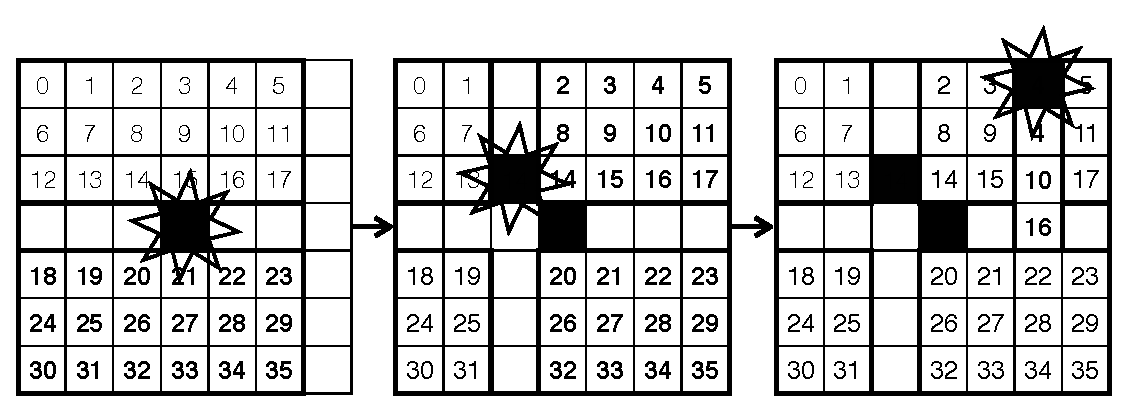
\includegraphics[width=75mm]{Figs/Hybrid.eps}
  \caption{Example of Hybrid(2D+1D) Sliding}
  \label{fig:hybrid-sliding}
\end{figure}

Thus, a hybrid sliding method can be expressed with the set of sliding 
methods and the order of their applications. As described in
Subsection\ref{sec:comparison}, the higher order sliding methods incur
lower message collisions but the number of failure able to
handle is smaller. Thus, the order of sliding methods to be applied in
a hybrid method should be a descending order of the degree of sliding
method. Hereinafter, a hybrid method will be expressed as
``hybrid(2D+1D+0D),'' for example, meaning 2D sliding is applied
whenever it is possible, then 1D sliding method is applied, and
finally 0D sliding method is applied. Since 0D sliding method can be
applied in any circumstances, any hybrid method should have 0D sliding  
method as a last resort. In this paper, a hybrid sliding method
combining all possible sliding methods with the descending order of
degrees is also denoted as ``hybrid(all)'' for short. Another hybrid
method combining all possible methods except $X$ is denoted as
``hybrid(-$X$).''  

In the next section, some simulation results will be shown followed by
an evaluation section on the K computer, BG/Q and TSUBAME
2.5\cite{tsubame}. One may 
argue that the numbers (percentages) of failed nodes simulated and
evaluated int this paper are too many and  not realistic. However,
those simulations and evaluations are done to reveal the behaviour and 
characteristics of the proposed substitution methods. We believe that
the research on how to utilize spare nodes is a new frontier of fault
mitigation. 

\section{Simulation}\label{sec:sim}

Since the number of combination of failed nodes is the factorial of
the number of failed nodes, it is impossible to simulate all possible
cases especially when the number of nodes is large. Instead of the
exhaustive search, the simulation results shown in this section are
obtained with random sampling. 

Figure \ref{fig:100x100}, Figure \ref{fig:12x12x12} and
Figure \ref{fig:24x24x24} show this simulation results on 2D network
(5P-stencil, 100x100, 2D(2,1) spare node allocation, 3,340,000 random
cases), 3D network (7P-stencil, 12x12x12, 3D(2,1) spare node
allocation, 3,686,400 random cases) and 3D network (7P-stencil,
24x24x24, 3D(2,1) spare node allocation, 3,686,400 random cases),
respectively. Each graph compares hybrid sliding method (3 thick
lines, worst, average and best from top to down) and 0D
sliding (3 thin lines, similarly, worst, average and best from top to
down) method. ``Best'' in the legend means the lowest number of
message collisions, ``Worst'' means the largest number of collisions
and ``Average'' means the average of all cases. 

\begin{figure}[ht]
\centering
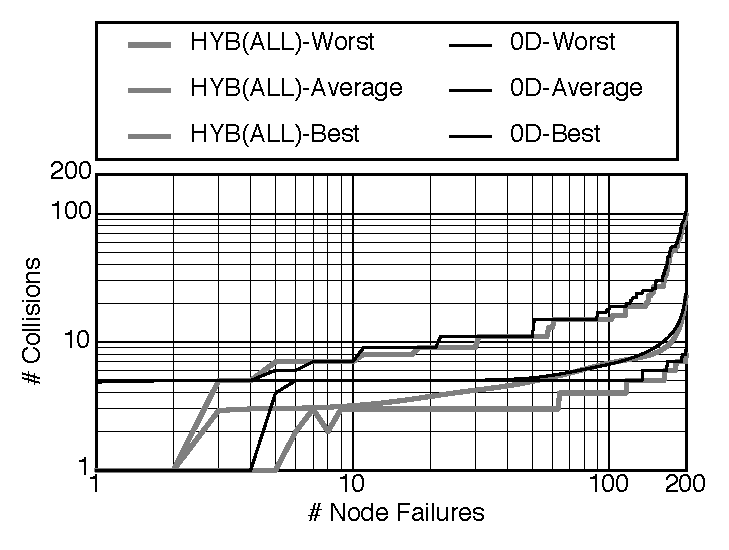
\includegraphics[width=80mm]{Figs/100x100.eps}
  \caption{Hybrid(all) vs. 0D, 2D Network (100x100), 2D(2,1) Spare Nodes}
  \label{fig:100x100}
\end{figure}

\begin{figure}[ht]
\centering
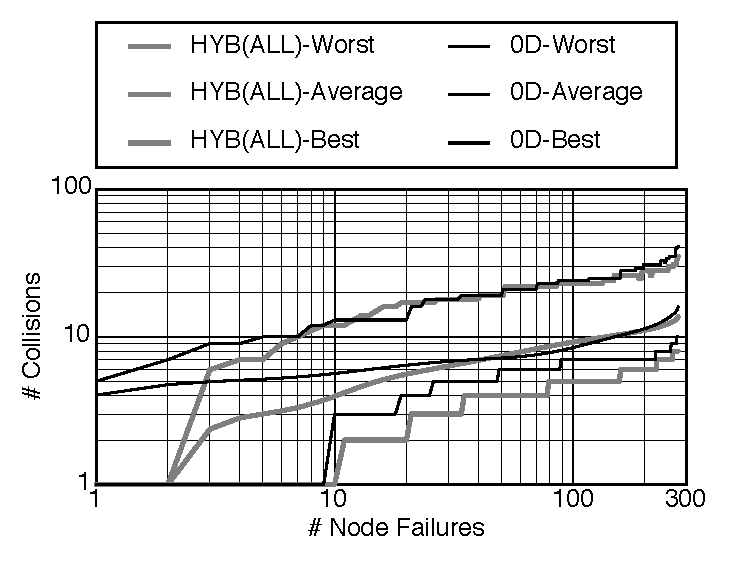
\includegraphics[width=80mm]{Figs/12x12x12.eps}
  \caption{Hybrid(all) vs. 0D, 3D Network (12x12x12), 3D(2,1) Spare Nodes}
  \label{fig:12x12x12}
\end{figure}

In the graphs in Figure \ref{fig:100x100} and Figure
\ref{fig:12x12x12}, hybrid sliding method outperforms 0D sliding
method in terms of best, average and worst cases in the smaller number
of node failures. 
In Figure \ref{fig:24x24x24}, however, the hybrid method outperforms 0D
sliding not so much as in the cases of 100x100 and 12x12x12. Comparing
the worst numbers, 0D sliding is better in the range of the number of
node failures between 9 to 261. Comparing the average numbers, 0D
sliding is better in the range of the number of node failures between
48 to 739.

\begin{figure}[ht]
\centering
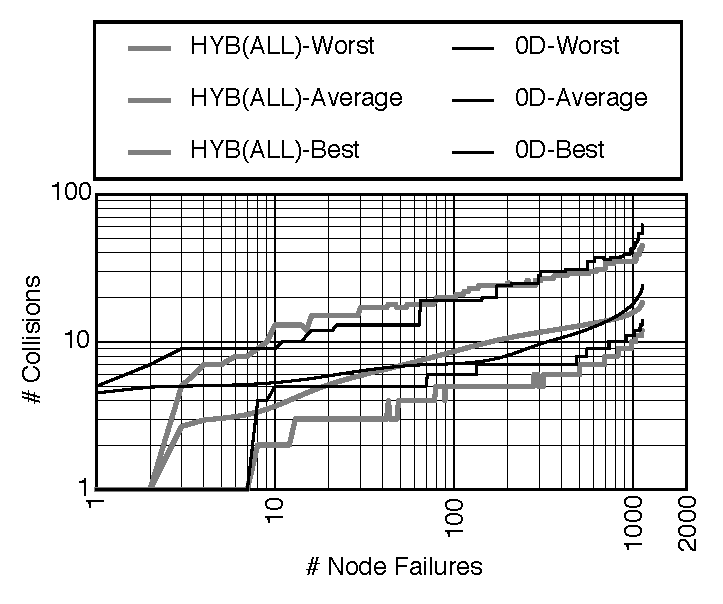
\includegraphics[width=80mm]{Figs/24x24x24.eps}
  \caption{Hybrid(all) vs. 0D, 3D Network (24x24x24), 3D(2,1)
    Spare Nodes}
  \label{fig:24x24x24}
\end{figure}

It is obvious that a stencil communication matches with a Cartesian
network if the degree of the network is equal to or higher than the
degree of the stencil communication. When a sliding method higher than
0D takes place, the network links connecting the nodes adjacent to the
{\it sliding planes} can result in message congestion. Here, {\it
  sliding plane} is defined as the planes which surrounds the sliding
nodes, except 0D sliding. The number of nodes (or the size of area of
the plane) adjacent to the 1D sliding plane is smaller than that of 2D 
sliding. Although the maximum number of message collisions of 1D
sliding and 2D sliding are the same, the number of collisions of 2D is
bigger than 1D. So, succeeding substitution may add
more message collision(s) to the nodes. From this viewpoint, 1D sliding
might be better than 2D sliding. Based on this idea, hybrid(-2D) or
hybrid(3D+1D+0D) might outperform hybrid(all).

Figure \ref{fig:24x24x24-hyb-2d} shows the simulation results of
hybrid(all), already shown in Figure \ref{fig:24x24x24}, and
hybrid(-2D) to compare. In this figure, the lines of hybrid(-2D) 
are thick. When attentions is paid to the average lines, hybrid(all)
outperforms hybrid(all) at the rages at the left most part, from 1 to
19, and the right most part, from 993 to 1128. Middle part, however,
hybrid(-2D) performs very well.

\begin{figure}[ht]
\centering
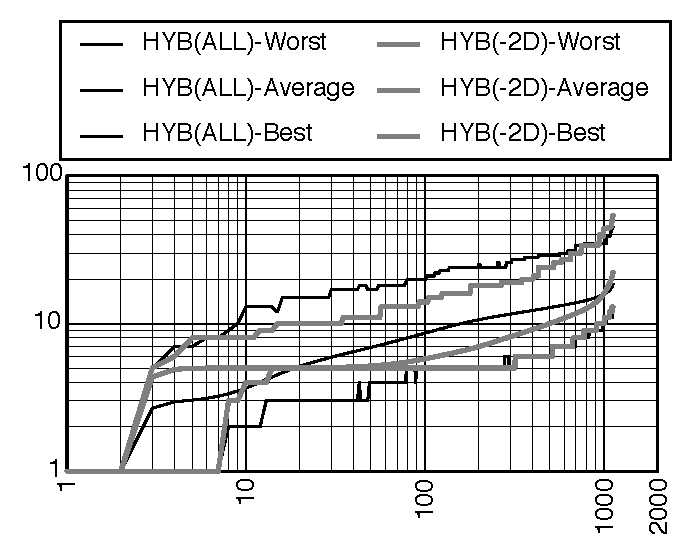
\includegraphics[width=80mm]{Figs/24x24x24-HYB310.eps}
  \caption{Hybrid(all) vs. Hybrid(-2D), 3D Network
    (24x24x24), 3D(2,1) Spare Nodes}
  \label{fig:24x24x24-hyb-2d}
\end{figure}

Figure \ref{fig:sel-rate} shows the rates of which sliding methods are
used in the sampling set. Figure \ref{fig:sel-rateA} shows the
accumulated selection rate. As shown in these figures, the first two
node failures are substituted by using the 3D sliding method. 2D
sliding method dominates until 38 node failures. Then, 1D sliding
method take over until 915 node failures. Finally 0D sliding method takes
the rest. As shown in Figure \ref{fig:sel-rateA}, when all the spare
nodes are substituted, 0D, 1D and 2D sliding methods occupy 25\%,
71\%, and 5\% respectively. 

\begin{figure}[ht]
\centering
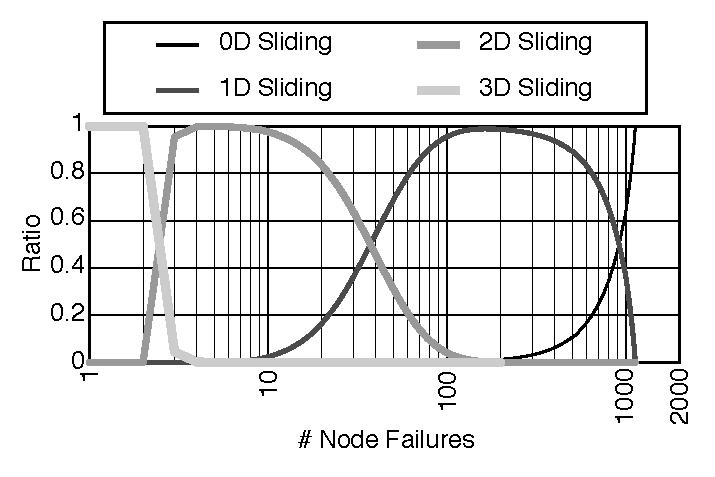
\includegraphics[width=80mm]{Figs/HYB-24x24x24-Sel.eps}
  \caption{Selection Rate of Hybrid(all) Sliding, 3D Network
    (24x24x24), 3D(2,1) Spare Node Allocation}
\label{fig:sel-rate}
\vspace{5mm}
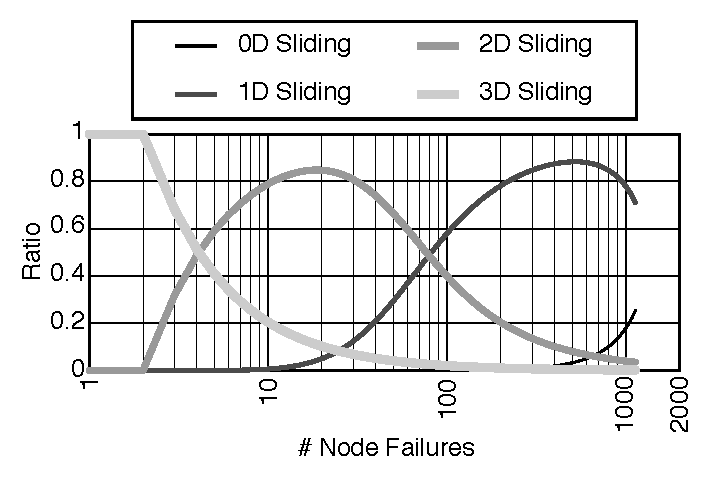
\includegraphics[width=80mm]{Figs/HYB-24x24x24-SelA.eps}
  \caption{Accumulated Selection Rate of Hybrid(all) Sliding,
    3D Network (24x24x24), 3D(2,1) Spare Node Allocation}
\label{fig:sel-rateA}
\end{figure}

\section{Evaluations on K, BG/Q and TSUBAME 2.5}\label{sec:eval}

In this section, the sliding methods described so far are evaluated by
using the actual supercomputers: the K computer
JUQUEEN\citep{JUQUEEN}, a BG/Q machine, and TSUBAME 2.5
listed in Table \ref{tbl:top5-network}.
This experimental campaign will characterize the difference
between the theoretical analysis and observed practical consequences.

The proposed sliding methods have been explained and discussed by
using a 2D Cartesian network, however, the actual physical network can
be more complex, having 5 or more number of dimensions, as shown in
Table \ref{tbl:top5-network}. Even if users
require their jobs to run in 2D node spaces, those 2D node spaces
are folded to fit in the actual network topologies. On the K computer,
any 2D Cartesian node planes are mapped to the 6D Tofu network so that
the neighbor relationship of the 2D or 3D Cartesian topology can be
preserved. On the BG/Q system, the node-rank mapping is the user's
responsibility. To preserve the neighbor relationship of the 2D or 3D
Cartesian topology, ``snake-like pattern'' is
recommended\citep{BGQ-softdev}. On TSUBAME 2.5, the physical node
space is one dimensional, dare to say. Anyhow, the
mapping or folding of users' topologies to fit into a physical network
topologies may affect the communication performance in different ways
discussed so far.

Also in this paper, we have focused our analytical effort on the
maximum number of message collisions, which has the implicit
assumption that all messages are sent from nodes simultaneously,
thereby always resulting in collisions if their path follows the same
link. However, the number of message that can be sent simultaneously
is dependent on network hardware features (i.e. the number of
DMAs). When the maximum number of simultaneous sends is one, for
example, the number of collisions is reduced.

\begin{table}[htb]
\centering
\caption{K, BG/Q and TSUBAME 2.5}
\label{tbl:machines}
{\small
\begin{tabular}{c|c|c|c|c}
\hline
Machine & Topo. & \# DMAs &\multicolumn{2}{c}{Ratio to 1 Msg. Sending}\\
Name & &  & 5P-Stencil & 7P-Stencil \\
\hline
K & 6D Cart. & 4 & 1.7 & 3.7 \\
BG/Q\cite{Chen:2011:IBG:2063384.2063419} & 5D Cart. & 10 & 1.1 & 1.3 \\
TSUBAME & FatTree & 1$^{\dagger}$ & 4$^{\ddagger}$ & 6$^{\ddagger}$ \\
\hline
\multicolumn{5}{l}{\footnotesize $\dagger$ TSUBAME 2.5 has 2 IB
  networks but only one of them is used} \\
\multicolumn{5}{l}{\footnotesize ~~~to avoid
  interference with the other jobs.} \\
\multicolumn{5}{l}{\footnotesize $\ddagger$ Estimated values.} \\
\end{tabular}
}
\end{table}

Table \ref{tbl:machines} lists some characteristics of the K computer,
BG/Q and TSUBAME 2.5. The K computer has 4 DMA engines and up to 4
messages can be sent simultaneously. BG/Q has 11 FIFOs and up to 10
messages can be sent simultaneously. The network of TSUBAME 2.5 is
Infiniband\cite{infiniband}. Although TSUBAME has two Infiniband HCAs
on a node, one of them is used in this paper to avoids the
interference with the other jobs. So, TSUBAME 2.5, in this case, can
sent only one message at a time. 

The rightmost two columns of this table show the ratios to send
multiple messages simultaneously, four messages with 5P-stencil, six
messages for 7P-stencil, based on the time to sent one message. These
values, except TSUBAME 2.5, are measured by our program. In
theory, 5 message collisions, for example, means the communication
time gets slower 5 times. On the K computer, only 3 times
slower communication time was observed because simultaneous 4 message
sending takes 1.7 times of the time of sending one message ($3 \approx
5/1.7$)\cite{Hori-EuroMPI2015}. One possible reason to explain this
slowness (1.7 with 5P-stencil and 3.7 with 7P-stencil) is the
insufficient bandwidth between the memory and network controller chip. 

In the following subsection, the evaluation results of the K computer
and BG/Q are shown. And then, evaluation results of TSUBAME 2.5 are
described. This is because they have Cartesian network topologies
while TSUBAME 2.5 has FatTree network topology. And the behaviour of
the K and BG/Q is very different from that of TSUBAME 2.5.

\subsection{Evaluations on K and BG/Q}

\subsubsection{Stencil Communication}

Figure \ref{fig:k-stencil} shows the simulation results on the
3D(12x12x12) network and the evaluation results of the K computer with
the 12x12x12 node allocation. Spare node are allocated in the way of
2D(2,1). Message size of 4MiB is used on the K computer
evaluations. The upper graph in this figure shows and compares the
results using hybrid(all) sliding method, and the lower graph shows
the results of using hybrid(-2D) sliding method. The 768 failure
patterns (the set of failed nodes) are chosen from the worst cases in
the simulation.

\begin{figure}[ht]
\centering
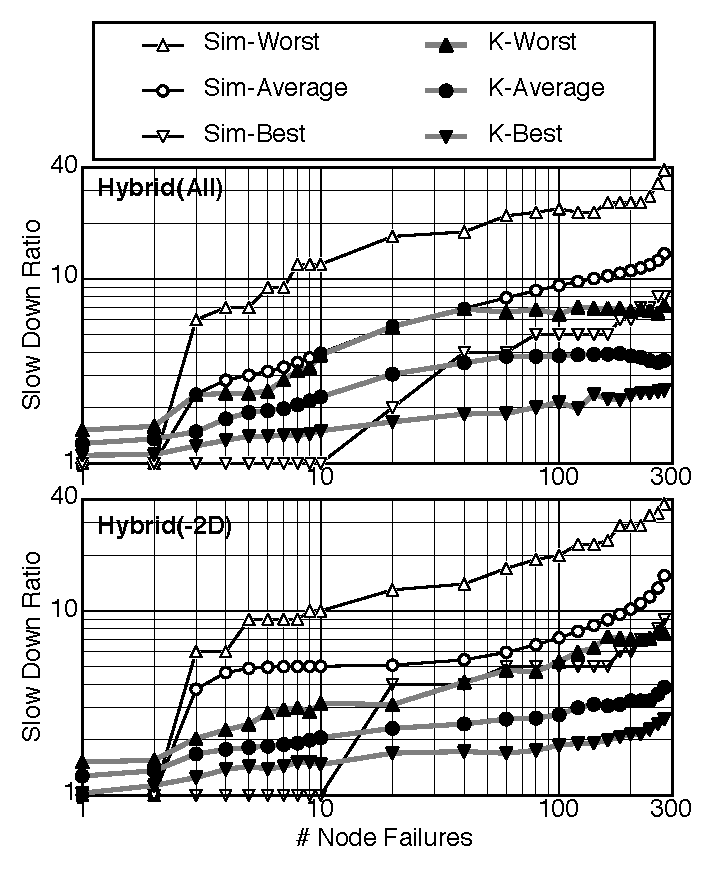
\includegraphics[width=80mm]{Figs/K-Stencil.eps}
  \caption{Stencil Communication on K (12x12x12), 3D(2,1) Spare Node
    Allocation}
  \label{fig:k-stencil}
\end{figure}

As shown in both graphs, the average lines observed on the K computer
is almost always better than the result of the simulations. This is
considered as the actual network degree of the K computer (6D) is
higher than the degree of the simulation (3D). The links provided by
the additional dimensions give the paths to bypass resulting lower
message collisions. Comparing the best lines, the simulation
outperforms in the rage of less than or equal to 10 node
failures. This is because of the sampling effect, the number of
simulation cases are much bigger than that of evaluation and the best
cases found in the simulation could not be found in the
evaluations. The same situation happens on the worst cases.

To compare hybrid(all) and hybrid(-2D), Figure \ref{fig:k-comparison}
shows the evaluation results of them (the same data used in Figure
\ref{fig:k-stencil}). The effect of hybrid(-2D) shown in this figure
is very similar to the one found in Figure \ref{fig:24x24x24-hyb-2d}. 

\begin{figure}[ht]
\centering
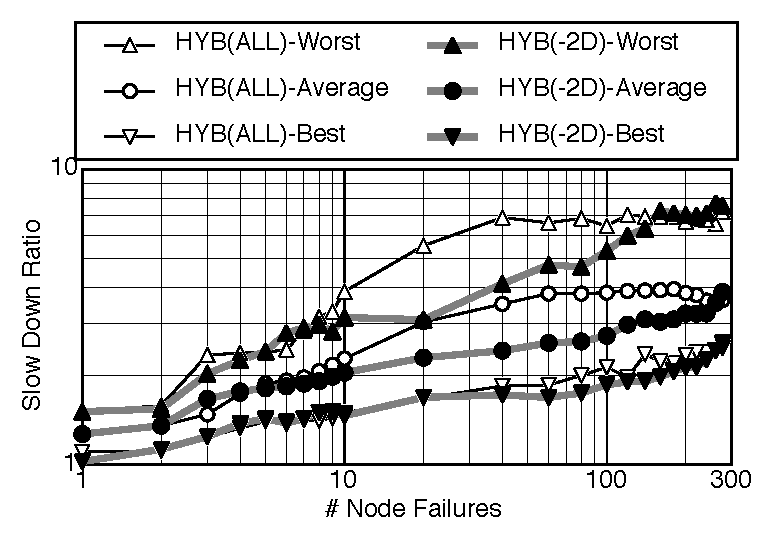
\includegraphics[width=80mm]{Figs/K-comparison.eps}
  \caption{Hybrid(all) vs. Hybrid(-2D) on K (12x12x12), 3D(2,1) Spare Node
    Allocation}
  \label{fig:k-comparison}
\end{figure}

Figure \ref{fig:bgq-stencil} shows the simulation results on the
3D(16x8x8) network and the evaluation on BG/Q computer with the 16x8x8
node allocation. Spare nodes are allocated in the way of
2D(2,1). Message size is 4MiB, the same as above cases on the K
computer. As in the previous graphs, the upper graph in this figure
shows and compares the results using hybrid(all) sliding method, and
the lower graph shows the results of using hybrid(-2D) sliding
method. Here again, the 768 failure patterns (the set of failed nodes)
are chosen from the worst cases in the simulation.

\begin{figure}[ht]
\centering
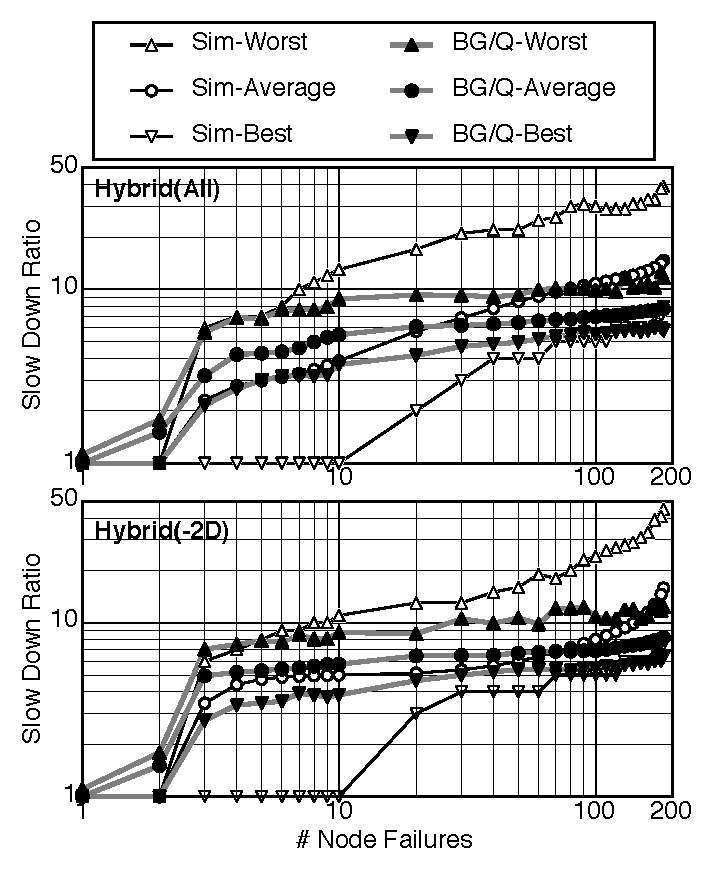
\includegraphics[width=80mm]{Figs/BGQ-Stencil.eps}
  \caption{Stencil Communication on BG/Q (16x8x8), 3D(2,1) Spare Node
    Allocation}
  \label{fig:bgq-stencil}
\end{figure}

Comparing the BG/Q results and the K computer results (Figure
\ref{fig:k-stencil}), the differences between the evaluation and the
simulation in the range of less than or equal to 10 node failures are
very small. This might come from the fact of that the network degree
of the BG/Q (5) is less than the degree of the K computer (6) and/or
that the network topology of BG/Q and the K computer are different.
The BG/Q network topology is full 5 dimensions, while the K computer,
the last three dimensions (A,B,C links out of X,Y,Z,A,B,C) are limited
more frequently, and to form a 2x3x2 subnetwork unit (Tofu unit).

\begin{figure}[ht]
\centering
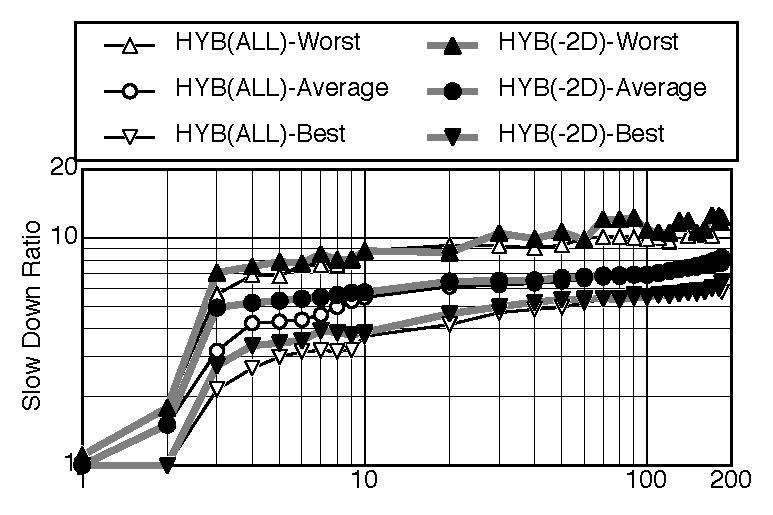
\includegraphics[width=80mm]{Figs/BGQ-comparison.eps}
  \caption{Hybrid(all) vs. Hybrid(-2D) on BG/Q (16x8x8), 3D(2,1) Spare
    Node Allocation}
  \label{fig:bgq-comparison}
\end{figure}

Figure \ref{fig:bgq-comparison} shows the evaluations of hybrid(all)
and hybrid(-2D) (the same data used in Figure
\ref{fig:bgq-stencil}). Unlike the case on the K computer (Figure
\ref{fig:k-comparison}), the difference between hybrid(all) and
hybrid(-2D) is very small.

\subsubsection{Collective Communication}

Up to now, the peer-to-peer (P2P) communication performance in
5P-stencil communication pattern has been the primary focus. In this
subsection, we will extend to the case of collective communication
performance.
The communication patterns of collective communications are more
varied that the stencil pattern, thereby providing a wider insight
about less regular P2P communication patterns as well.

On the K computer, the Tofu network supports hardware barrier. The
other various collective communications are tuned so that the best
performance can be obtained based on the Tofu network
characteristics\cite{sumimoto-k}. The tuning of collective protocols
is also very important for the Cray's Gemini
network\cite{Pena:2013:ATM:2488551.2488564}. However, it is very
difficult to predetermine optimized collective protocols for any
possible set of node failures. 

In order to tune collective protocol for the Tofu netwotk, each MPI
collective communication has some conditions for the physical shape of
the communicator. Some of the conditions come from the special protocol
tuned for the Tofu network, and the others come from implementation
issues. When a substitution is made for a failed node, one or more of
these conditions cannot be met and generic algorithms are used. Thus,
the performance of the collective communication can degrade much more
than that of the stencil communication, because the special tuned
protocols cannot be applied in addition to the collision issue.

\begin{figure}[ht]
\centering
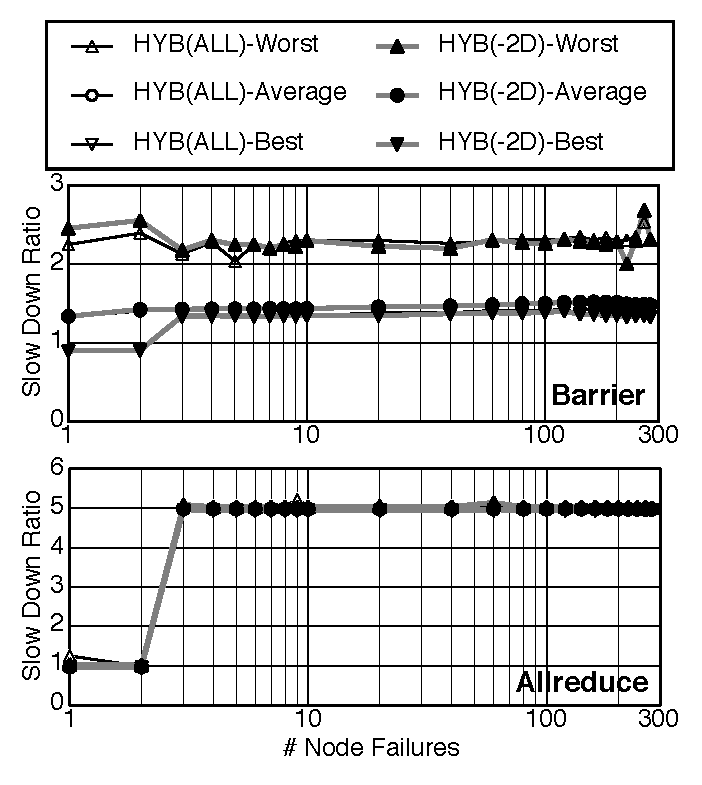
\includegraphics[width=80mm]{Figs/K-Collective.eps}
  \caption{Barrier and Allreduce on K (12x12x12), 3D(2,1) Spare Node
    Allocation}
  \label{fig:k-collective}
\end{figure}

Figure \ref{fig:k-collective} shows the relative performance of
barrier (upper graph) and allreduce (lower graph) collective
communication based on the performance of no substitutions are
made. Nodes of the evaluation job are allocated in 3D(12x12x12) and
the sampling set is the same as the evaluation of stencil on the
K computer in the previous subsection. The message size of allreduce
is 64KiB. 

On the allreduce case, the slowdown cannot be seen with one node
failure and two node failures. In this evaluation, hybrid sliding
methods are used and spare nodes are allocated in 2D(2,1), so 3D
sliding method can be applied up to two node failures. The sliding
method having the largest degree happens no message collision as
described in Section \ref{sec:comparison}. And this property of
the sliding method with the largest degree does not break the
conditions where the optimized allreduce protocol on the K computer
can be applied. 

\begin{figure}[ht]
\centering
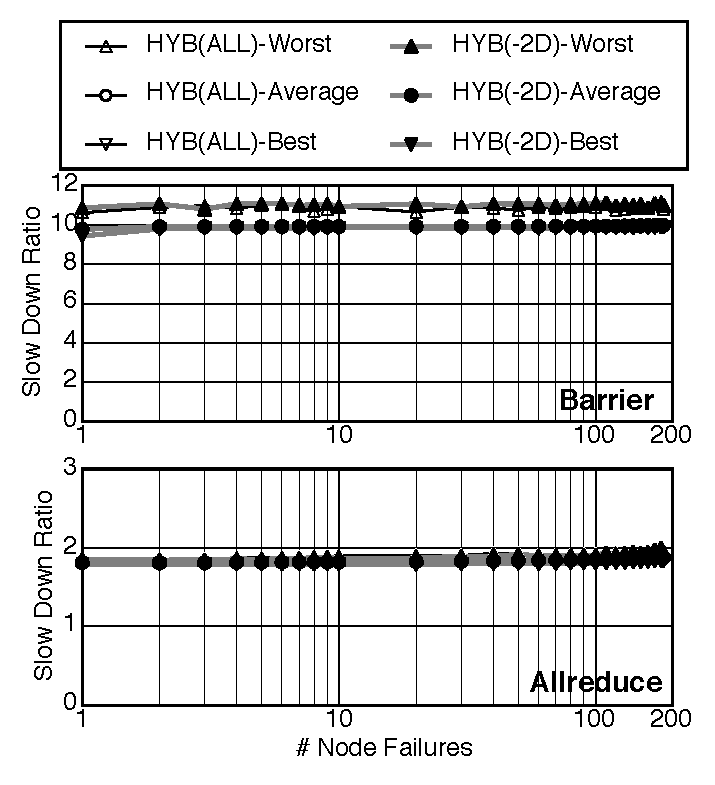
\includegraphics[width=80mm]{Figs/BGQ-Collective.eps}
  \caption{Barrier and Allreduce on BG/Q (16x8x8), 3D(2,10 Spare Node
    Allocation}
  \label{fig:bgq-collective}
\end{figure}

Figure \ref{fig:bgq-collective} shows the barrier and allreduce
performance on BG/Q. We found that the collective performance on
the node set having a spare node set is slower than the cases without
having any spare node. 8.2 times slower with the barrier operation and
1.8 times slower with the allreduce operation on BG/Q. Such slowdown
cannot be seen on the K computer. This graph shows the slowdown ratio
based on the time of the cases having spare nodes.

To make sure, we evaluated the barrier performance
without the snake-like pattern mapping. When the spare nodes were
allocated on one specific physical dimension out of the 5 dimensions
of the BG/Q network, such barrier performance degradation could not be
seen. However, when one node was excluded from {\tt MPI\_COMM\_WORLD},
then the barrier performance was slowed down to one tenth. Thus, the
best way is to allocate spare nodes according to the network topology
and then apply the snake-like pattern to the node space without spare
nodes. 

Unlike the K computer collective cases, the barrier and allreduce
performance of BG/Q is quite stable over the number of node failures
independent from hybrid method. The 3D sliding method did not help to
improve the situation.

\subsection{Evaluations on TSUBAME 2.5}

We ran the same evaluation programs on TSUBAME 2.5, 7x7x7 node
space with 2D(2,1) spare node allocation. Unlike the K and BG/Q cases,
we could not see any significant slowdown. The communication
performance is almost constant within the range of 1.0 to 1.2 over the
sliding method and the number of node failures, no obvious
correlation. To make sure of this phenomenon, we additionally
evaluated the sliding methods with random node-rank mapping. As far as
we tried, no obvious performance degradation can be seen.

One possible reason of this phenomenon is that the network topology of
TSUBAME 2.5 is 2-stage FatTree. The node space is expressed in one
dimensional way for the sake of convenience. However, there is no
significance on the node numbers of the nodes connecting to the same
``edge'' switch. Any changes on node-rank mapping on those nodes have
no effect. 

The other factor of this phenomenon is that the network of TSUBAME 2.5
is Infiniband. Indeed, TSUBAME 2.5 has two network set so that the
communication bandwidth can be doubled by utilizing them in the
multi-rail way\cite{1392963}. One of the network sets is also used for
Lustre file system and it is likely to have I/O traffics of the other
jobs. So we decided to use the other network set to 
avoid the interference with the other jobs. Each Infiniband HCA has
one DMA engine and, unlike the K computer and BG/Q, only one message
can be sent from an HCA at a time. In a stencil communication, in
theory, multiple messages can be sent simultaneously, however, TSUBAME
2.5 has the capability of sending only one message in this case. This
situation is very different from the K computer able to send up to 4
messages and BG/Q able to send up to 10 messages simultaneously (Table
\ref{tbl:machines}). This leads to have less messages in the network
and to have less chance to have message collisions. This may happen
also with the collective communications.

\section{Related Work}\label{sec:related-work}

Ferreira {\it et al.} indicated that dual hardware redundancy while
utilizing only 50\% of the hardware resource, might be under some
assumptions more efficient than the traditional checkpoint and restart
method in Exascale systems This redundancies can be thought of as
spare nodes. The difference is that the redundant nodes are {\it
  hotter}-standby than the hot-standby nodes waiting for the
intermediate computational results. The spare nodes can be substituted
for the failed nodes, and they can almost immediately take over the
computations.

Domke {\it et al.} showed the difference in communication performance
between the presence or absence of network failure (link or switch)
over different network topologies and routing
algorithms\citep{Domke:2014:FND:2683593.2683659}. They analyzed the
communication performance degradation when network links or switches
failed; this was done by simulation using TSUBAME 2.0. In the K
computer, the Tofu direct network has redundant routes to bypass
failed nodes. However, a job is aborted and resubmitted by the
operating system if it uses a failed part. In this work we focus on
node failures rather than network failures. There is a
long way to go until we reach the goal where any kind of failures,
node and/or network, can be mitigated.

Brown {\it et al.} proposed a visualizing system of message traffics
in a communication network\cite{7384355} and they succeeded to
identify hot-spots. In their case study using the samplesort program
running on TSUBAME 2.5, 5\% performance gain was obtained by avoiding
the hot-spots. Conversely speaking, their paper reveals that finding
an optimal node-rank mapping to level hot-spots according to network 
topology and communication pattern of an application is not an easy
task.

\section{Discussion}

\subsection{Node Utilization in a Multijob Environment}
\label{label:multi-job}

Most supercomputers use a batch scheduling system, in which many jobs
run simultaneously. The spare node percentages shown in Figure
\ref{fig:sparenode-percentage} are for individuals jobs, not
systems. If a machine has one million nodes and 100 jobs are running
(for simplicity, assume that these jobs each require 10,000 nodes),
then the overhead cost of spare nodes can exceed 10\%.

The possibility that a job has a failed node is proportional to the
number of nodes assigned to the job and execution time. Thus, the
number of spare nodes must also be proportional to the number of nodes
assigned and execution time. Therefore, the number of spare nodes
allocated by the proposed method may be excessive when only a small
number of nodes are required by a given job. Ideally, the curves shown
in Figure \ref{fig:sparenode-percentage} would be a horizontal line at
the height determined by node failure rate, if the execution times are
the same.

\begin{figure}[ht]
\centering
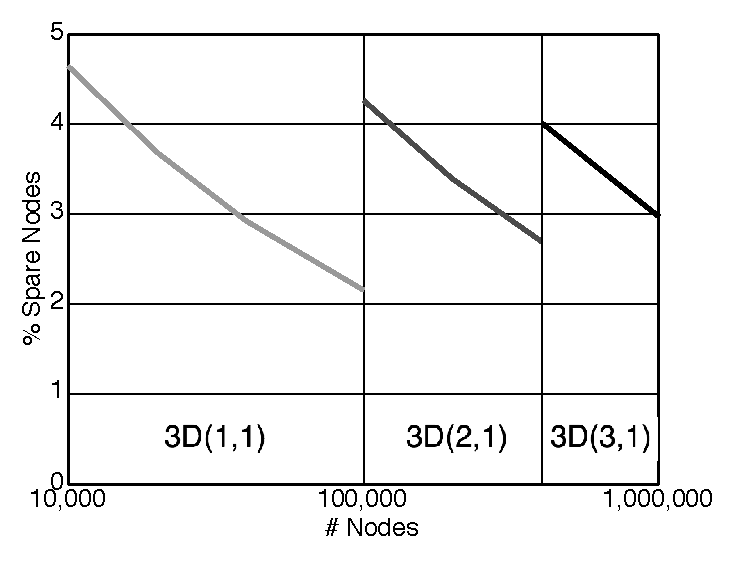
\includegraphics[width=55mm]{Figs/R-SpareNodes-combo.eps}
  \caption{Combinations of spare node allocation methods}
  \label{fig:combo-percentage}
\end{figure}

Figure \ref{fig:combo-percentage} shows a countermeasure for
this. Large jobs should have a higher-order spare node allocation
method, and smaller jobs should have a lower-order method; this will
allow the spare node percentage to approximate a horizontal line. In
the example shown in Figure \ref{fig:combo-percentage}, the spare node
percentage is kept in the range from 2\% to 5\% by using a combination
of the 3D(2,1), 3D(2,1), and 3D(1,1) methods.

\subsection{User-level vs. System-level Substitutions}

So far in this paper, we have considered methods in which the spare
nodes are allocated by the job. We would like to develop a framework
that uses something like ULFM and that framework replaces
faulty nodes with spare nodes, so that users do not need to be
concerned with how failures are handled. When spare nodes are
allocated and substitutions are determined by user programs, this is
called as {\it user-level substitution}; when this is done at a lower
system software level, it is called {\it system-level substitution}.

With user-level substitution, the user program is also invoked at each
spare node, and it waits in hot-standby mode for the data to migrate
from the failed node. This means that calling {\tt MPI\_Comm\_spawn}
is not required. On the other hand, system-level substitution can
reduce the percentage of spare nodes, because spare nodes can be
shared by several jobs. For example, spare nodes can be allocated at
the boundaries of jobs, and these can be used to replace failed nodes
on both sides of the boundary. However, it is not possible to have
spare nodes on hot standby, as with user-level substitution. If the
spare nodes are not adjacent to the job in which they are needed, this
can result in uncontrollable message collisions with other jobs, and
unexpected communication performance degradation.

\subsection{Job Resubmission vs. Fault Mitigation}

One may argue that a job can be aborted and then resubmitted using a
checkpoint, instead of mitigating the fault. In this way, the problem
of utilizing spare nodes and the degradation of communication
performance, described above, can be avoided. Job resubmission,
however, may incur a long turnaround time, especially when the system
is heavily loaded, and user-level fault mitigation techniques, such as
those described in \citep{Davies:2011:HPL:1995896.1995923}, cannot be
utilized. When considering which is better, there are many aspects to
be considered. In this paper, we considered only the effect on
communication performance. It is still an open question if it is
better to resubmit a job or mitigate the fault.

\subsection{Worm Eaten Node Space}

So far in this paper, a obs is allocated with a node space where there
is no node failure at the beginning. Usually, when a node failure
happens, the failed node is to be replaced with a new healthy
node. To replace the failed node, firstly this node is unplugged from
a rack and or chassis and then sanity node is plugged in. When a node
is unplugged from a rack or chassis and if its network is a direct
network, then the switch associated with the node is also gone. Thus,
unplugging a node unintentionally simulates a switch failure, even
with the assumption of no network failure.  When a
switch failure happens, network routing must be changed to bypass the
failed switch and this may affects the other running jobs. So, the
physical node replacement cannot take place soon after the node
failure happens. 

It is expected that MTBF is increasing in the future. And there will
be the case where node failure happens much more frequently. Thus, the
number of node failures will increase with in the interval of
repairing nodes. This may result in the situation where large jobs
might be allocated with a ``worm-eaten'' node space, instead of having
all healthy nodes. In this case, node substitution methods described
in this paper and/or algorithms to find an optimal node-rank
mapping must be applied from the beginning of job execution. Therefore
we believe the research on node substitution and the algorithm to find 
(sub)optimal node-rank mapping will be very important. This is left
for our future work.

\section{Summary and Future Work}

In this paper, we considered methods for allocating spare nodes and
replacing failed nodes in jobs whose rank-node mapping is critical to
performance. We compared these methods in terms of
communication performance following substitutions. The substitution
methods are 0D, 1D, 2D, higher sliding methods. In the Stencil 
communication, the higher the order of the sliding method, the fewer
message collisions but more failure distributions are unrecoverable
for lack of spares. Thus, a combination of these methods would seem
to be the best strategy. We also extended the evaluation to widely
used collective operations. 

Utilizing spare nodes influences various fields in high-performance
computer design, hardware and software. As shown in the evaluations,
a network topology plays an important role. It is expected that the
communication performance degradation found in the substitutions can
be relaxed by having a dynamic routing. The mapping of applications'
communication patterns and optimizations of collective
communication patterns to fit in the available network topology becomes
very difficult with the presence of failed node substitutions. Because 
there is no regular pattern where node failure happens and the
number of node failure patterns are explosive. Therefore the
assumption to have spare nodes has a significant impact on hardware
and software design.

The research on this failed node substitution with spare nodes has
just begun. We will continue investigating on this research topic.

\begin{acks}
We thank Dr. Norbert Attig at J\"{u}lich Supercomputing Center for
allowing us access to the JUQUEEN platform. We also thank Dr. Franck
Cappello, at Argonne National Laboratory, for his useful
comments. 

A part of the results in this paper is obtained by using the K
computer at the RIKEN Advanced Institute for Computational
Science (HPCI Project ID {\tt hp150240}).
\end{acks}

\begin{funding}
This research is partially supported by the CREST project of
the Japan Science and Technology Agency (JST).
\end{funding}

\bibliographystyle{SageV}
\bibliography{ref,hori}

\end{document}
